\documentclass[12pt, letterpaper]{article}
\usepackage{makecell}
\usepackage{graphicx}
\usepackage{float}
\usepackage{enumitem}
\usepackage{amssymb}
\begin{document}

\begin{titlepage}
    \centering
    {\Large EECS 401/402 - Senior Design \par}
    \vspace{1cm}
    {\huge\bfseries Web-Based Interactive Music Education Tool\par}
    \vspace{1cm}
    {\Large Design Report\par}
    \vfill
    {\large
    Davis Akard \\
    Connor Finley \\
    Viktor Potter \\
    Ryan Thweatt \\
    Jason West\par}
    \vspace{1cm}
    {\large
    Course: EECS 401/402 \\
    Instructor: Jian Huang\par}
    \vfill
    {\large May 1, 2026 \par}
\end{titlepage}

\section*{Executive Summary}
The goal of our senior design project is to create a web-based interactive music education tool that supports college-level music theory and ear training. Our tool is inspired by the existing BriFormer platform used in some UTK music courses and other applications, but it aims to address its major drawbacks with the user interface while still keeping its strengths. Our application will provide a clean and user-friendly interface that will allow users analyze real music and their phrase structure in diagram form. These main requirements were decided based on feedback from UTK music faculty and students who have used BriFormer. Their primary concerns were that the existing tool feels visually cluttered and difficult to navigate, especially for new users.

Technically speaking, this is implemented as a full-stack web application using Next.js with React and TypeScript on the frontend and Supabase as the backend for data storage/authentication. The frontend includes pages such as login, project dashboard, our improved BriFormer analysis view, and a sound-to-score conversion tool. The backend manages user accounts and saved projects, which converts to the frontend through Next.js API routes backed by Supabase. GitHub serves as our collaboration and version control platform. The application will work with YouTube to let users import and play music directly within the browser. This will go hand-in-hand with the BriFormer-style analysis tool so that students can mark sections, phrases, and other elements on top of a timeline.

Our project was delivered in three phases: development, testing/feedback, and deployment. During development, we implemented the account login and structure, our improved BriFormer tool, and sound-to-score conversion. In the testing/feedback phase, we met with two professors in the college of music. One professor was provided with the tool for their own use and the other professor was walked through the tool and its functionality. Both professors had solid ideas on how to improve the BriFormer tool. These ideas are outside the current scope of the project, but will be worked on in the future. Finally, in the deployment phase, we worked closely with the UTK music faculty to present our tool and discuss its use and practicality in the real world. By the end of the project, our expected result is an instructor-tested web application that is ready for possible further deployment and actually improves the usability and clunkiness of BriFormer-style music education tools.

% Remove page numbers from title page and TOC
\pagestyle{empty}

\tableofcontents
\listoftables
\listoffigures
\newpage

% Begin page numbering here
\pagenumbering{arabic}
\pagestyle{plain}

\section*{Problem Definition and Background}
\addcontentsline{toc}{section}{Problem Definition and Background}
At the University of Tennessee, Knoxville and elsewhere, instructors often rely on a combination of learning management systems (such as Canvas in UTK's example), outside music theory websites, and tools like BriFormer to implement music-related assignments. While these tools are useful, faculty and students have stated that the existing Briform-style interface can be difficult to navigate and visually cluttered, especially for new users. This means that students may struggle more with the tool than with the musical concepts they are meant to be learning, and instructors would have to spend extra time explaining the interface instead of focusing on the actual music concepts themselves. Therefore, the core problem is that current tools for musical analysis and ear training do not provide a user-friendly environment that fits into modern college music classes. For example, Briformer is explicitly designed around musical form. In an Open Music Theory worksheet on AABA and strophic form, students are instructed to ``Use the BriFormer web app to create a formal diagram'' and to click ``Create a new BriFormer using a YouTube link'' for specific recordings~\cite{omt-aaba}. These uses show that BriFormer might be able to be integrated into coursework, but they also highlight its limits: it mainly functions as a standalone diagramming tool with subpar integration into the workflow of students and teachers.

The primary people affected by this problem are music instructors and students in college-level education. Instructors need a reliable way to assign tasks and to review student work efficiently across multiple class sections, class types, and class periods. Students need an accessible tool where they can import real music examples, annotate form and phrase structure and other musical concepts. Some other people that may be impacted could include department administrators or advisors, who care about consistency across many different courses, and the music department's technical staff, who have to support authentication and data management for any new tool that handles student coursework.

The basic functions this design must perform are (1) allow users to load music from common media platforms (YouTube); (2) provide a timeline where students can mark sections, phrases, and other musical aspects; (3) allow users to export and share projects; and (4) provide a system for users to convert audio files to score notation. Additional features could include progress tracking and support for different types of exercises like ear training, rhythm, notation-focused or instrument-playing activities.

The tool will primarily be used in two environments: during instructor-led class activities and as assigned homework or studying. Instructors should be able to project the interface in a classroom to walk through a song's form with students, while students use personal laptops with headphones to complete individual assignments, possibly inside of class for attendance or outside of class for homework. For the backend environment, the system must operate in a web environment, handle multiple users at once, while ensuring basic security and privacy for user accounts. This means the design has to consider not only end users (students and instructors) but also aspects such as accessibility and browser support.

This project intersects music theory, ear training, and web-based learning. Students are expected to work with concepts such as strophic/AABA form and harmonic analysis, as described in open resources like \emph{Open Music Theory}. This is described as ``a natively-online open educational resource intended to serve as the primary text and workbook for undergraduate music theory curricula''~\cite{omt}. Our tool aims to enforce these resources by providing an environment where students can apply those concepts to real music that they love or teachers assign, rather than only to musical scores.

Prior tools and products have provided context for our design. Teoria, for example, is described as a ``Web site dedicated to the study of Music Theory. Articles, reference, interactive exercises''~\cite{teoria-main}. A separate review notes that ``Teoria is a platform for learning music theory \& improving your ear'' and that its tutorials are ``accompanied by exercises which enable students to gain fluency with each concept''~\cite{teoria-review}. Similarly, musictheory.net states, ``introductory and intermediate music theory lessons, exercises, ear trainers, and calculators''~\cite{musictheory-main} are used. These platforms show that browser-based lessons and ear-training exercises may be effective, but they do not provide all the tools that students and teachers need in a user-friendly layout. Similarly, EarMaster markets itself as ``the ultimate app for ear training, sight-singing, and rhythm training'' with ``4000+ exercises for all levels''~\cite{earmaster-main}. EarMaster Cloud, a major music-education focused platform, is promoted as ``an all-in-one solution for schools, conservatories, choirs and private studios of any size''~\cite{earmaster-cloud}, with teacher and student management tools. However, these products can be locked behind paywalls or may not include all the features that students need for music theory and ear training.

All in all, this background suggests that there is a clear need for a web-based music education tool that combines the strengths of existing platforms and learning management systems, while addressing the concerns raised by instructors and students who have used BriFormer. Our project is intended to fill these gaps by providing a Briform-inspired interface but with UI and feature improvements so that the technology supports rather than holding back the learning of music theory and ear training.

\section*{The Requirement Specification}
\addcontentsline{toc}{section}{The Requirement Specification}
Our requirements, in order of priority, are: developing a fully functional web application, connecting a media platform to enable song manipulation, designing a BriFormer-like page for music education, managing user login credentials, and grading music assignments. We decided on these requirements by listening to feedback from professors and music theory students on their experiences with BriFormer.

\textbf{Application.} Having a working application, a way for users to interact with our product, is our number one priority. We plan to deliver a fully functional web application that users can access from anywhere. Our web app will host our BriFormer-like tool, allowing teachers and students to complete assignments and study music.

\textbf{Media.} Our project is a music education tool. Thus, our users need a way to import songs so that they can study music and learn from it. We are choosing to use YouTube's API, which allows users to select a video on YouTube and then analyze it, dissect it, and overall hone their skills.

\textbf{Design.} The number one complaint that BriFormer users possess is how clunky and unusable the design feels. We plan to keep the functionality of BriFormer while updating the UI to be intuitive for users. We want people to enjoy using our tool, rather than it being a chore. Alongside a better UI, we plan to add some more functionality to our tool so that users can take their music education to the next level.

\textbf{Login.} Users will need a way to log in to our web application to save their projects and access them from any device. We are still figuring out the best way to store user credentials; however, we plan to create a login page so that users can securely store their projects.

\textbf{Accessibility.} Users can share their projects with other users and these shared projects can be seamlessly picked up. Additionally, BriFormer projects and Sound-To-Score projects can be downloaded and exported to display results and retain offline access to the audio and visual effects without using the webpage. 

Overall, our requirements give us a clear focus when creating our music education tool. Our requirements are carefully chosen by feedback from teachers and students, and give us a path towards designing a music education tool that people will enjoy using.

\section*{Technical Approach}
\addcontentsline{toc}{section}{Technical Approach}
\subsection*{Project Space}
\addcontentsline{toc}{subsection}{Project Space}
Our project space consists of a frontend and backend space, as well as a synchronization method. The frontend space primarily consists of NextJS code. Each site component will have an individual file that defines it. Those components are then compiled into pages, with each page having its own folder and page.tsx file. The frontend space defines what the user is able to do on the site and how the user interface will facilitate it. 

The backend space will hold necessary user information, including login credentials, account type, classes enrolled/teaching, assignments or projects, etc. We need to have user accounts to fulfill our user requirements, so a strong backend is crucial. Whether we use a simpler approach with an external account system or a more customized approach with a backend provider, we will need to connect the back and front ends seamlessly with NextJS.

This project involves splitting of work among the group members. This necessitates a way to centralize and synchronize our work. We use GitHub to accomplish this. GitHub allows us to constantly have a “most recent” version of the site. It also ensures that any conflict caused by our separate work is quickly resolved and provides accountability for everyone committing their sections of the work themselves.

\subsection*{Functional Decomposition}
\addcontentsline{toc}{subsection}{Functional Decomposition}
\begin{figure}[H]
    \centering
    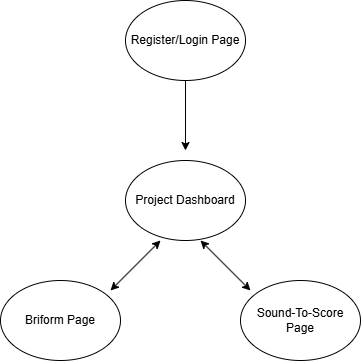
\includegraphics[width=0.5\linewidth]{images/402TechDia.drawio.png}
    \caption{Technical Diagram}
    \label{fig:tech401}
\end{figure}

The first functional unit of the website is the register and login page. On this page, the user will be prompted to either log in to an existing account or to create a new account. If a user needs to create an account, they will be directed to do so and receive a confirmation email to create the account. Then they will be redirected to the project dashboard. If a user already has an account and logs in, they will also be redirected to the project dashboard.

Once the user is at the project dashboard they are able to resume saved projects or create new projects. There are two styles of projects to choose from: BriFormer and Sound-To-Score. BriFormer projects allow users to study music form and phrase, while Sound-To-Score projects allow users to study the score notation of songs.

The BriFormer-style page takes inspiration from the site BriFormer. In this page, users will be able to make new projects in which they use a music audio file or a video to score the music and practice things like ear theory. They will also have the choice to save the project they finished, and if they want to continue a project, they can upload an existing saved project to resume where they left off.

Next, on the Sound-To-Score page the user selects a music audio file or a video and then the audio is converted to score notation and displayed on the webpage. Users are able to play the audio and score notation to study how sounds appear in score notation. They can see single staff, double staff, and all the different clefs. The information is also downloadable so that the score notation can be shared and accessed offline easily.

\subsection*{Key Design Decisions}
\addcontentsline{toc}{subsection}{Key Design Decisions}
There are several key design decisions we need to make throughout the process of this project. There are two major decisions surrounding the project space. The first is whether to use a web-based approach with NextJS (or similar language) or an application-based approach with a language like Python. Another decision is whether to use an external account system (such as using exclusively a YouTube/Google account) or a back-end like Supabase.

The rest of the major decisions deal with the design and structure of the program. One major decision is whether to support some form of auto-grading of assignments or if grading must be strictly manual from instructors. We must also consider if and how we want to integrate Spotify and/or YouTube, as well as how both can be used. Another major decision is whether we want to use a design inspired by BriFormer or make our own design that accomplishes similar functionality.

As we have progressed, two more key design decisions have presented themselves. The first is whether we want to support searching for YouTube videos to use as the improved BriFormer’s audio source or keep BriFormer’s method of simply pasting a link to the YouTube video. The second is whether we want to create a custom solution for the sound-to-score portion of the project or implement existing tools.

\section*{Design Concepts, Evaluation, and Selection}
\addcontentsline{toc}{section}{Design Concepts, Evaluation, and Selection}
\subsection*{Web Application vs. Downloadable Application - Davis Akard}
\addcontentsline{toc}{subsection}{Web Application vs. Downloadable Application - Davis Akard}
When we first began crafting our design for a music education tool, we deliberated between two ways to bring it to users. We could either design a web application that users could connect to through a browser or make an executable that users would download and launch. Both ideas had their pros and cons; however, we ultimately decided on designing a web application. We went this route for multiple reasons, but the biggest reason was usability. One of our main focuses is usability, and a web application is much more usable than a downloaded application. Web browsers give users access to our tool by simply clicking on a link, whereas a downloaded application is harder to distribute, requires downloading, and is overall clunkier to use. We also decided on a web browser because it was a format that we were more comfortable with designing, implementing, and coding. HTML, CSS, and JavaScript are all relatively basic programming languages and something that we are either comfortable with or will become comfortable with quickly. Designing a downloadable application is something we are unfamiliar with, and designing one would take a lot more effort than a web application.

\subsection*{Offsite Login vs. Backend Provider - Ryan Thweatt}
\addcontentsline{toc}{subsection}{Offsite Login vs. Backend Provider - Ryan Thweatt}
Another important decision to make is how we want to handle the account system. We could use an exclusively external account system. This would involve taking advantage of existing accounts with the platform(s) we integrate into the app (eg., YouTube/Google or Spotify accounts). This would be very simple for users, as it is a common method of account creation. However, it does not allow for the same level of customization that using a backend provider like Supabase would. Using a backend provider would likely make it simpler to differentiate between student and instructor accounts and give us more flexibility in how we design the front end. In addition, we could link multiple offsite accounts (i.e., link both YouTube and Spotify accounts) to a user’s profile instead of being locked into one.

\subsection*{Auto-Grading \& Manual Grading vs. Strictly Manual Grading - Viktor Potter}
\addcontentsline{toc}{subsection}{Auto-Grading \& Manual Grading vs. Strictly Manual Grading - Viktor Potter}
One of the major design decisions for our product was whether assignments could be marked as autograded or manually graded by teachers, or if we would require teachers to grade their assignments with no option for autograding. For the choice of making teachers grade themselves with no option for autograding, it will be as simple as providing the teacher a box where they put the total possible score when creating an assignment, and then having them go back once a student submits an assignment to put in a grade themselves. When it comes to having an autograde system, we would have to make our own model for how assignments should be graded, as well as implement a way for teachers to adjust the autograding system. When it comes to these two alternatives for grading, the best decision for what we are making would be to only have manual grading enabled. As the time for our project is limited and along with all of the other functions that need to be built for the website, the time it would take to set up a proper autograding system would be too high compared to its overall importance to the project. The autograding feature may also be something that could cause teachers' headaches if we do not implement it properly, or if there are bugs within the autograding system that we fail to find. The time that would be spent making this feature would be utilized much better for optimizing the main components of the site and enhancing the user experience through a well-polished site instead of an autograding system. Unfortunately, grading integration as a whole has been scrapped due to the time constraints of this project. We had to prioritize creating an optimal BriFormer tool and sound-to-score tool instead of focusing on grading assignments. Users can export their projects and submit them separately for grading though.

\subsection*{Spotify Integration vs. YouTube Integration - Connor Finley}
\addcontentsline{toc}{subsection}{Spotify Integration vs. YouTube Integration - Connor Finley}
When considering how to allow users to import music into our application, we debated between integrating Spotify or YouTube. Spotify's API is extremely intuitive, and account login is simple through OAuth.  However, Spotify's API does not allow for streaming full songs, which is a major drawback for our application. Additionally, Spotify’s API requires users to have a Spotify Premium account. On the other hand, YouTube's API allows for full video streaming and does not require the user to have a YouTube account at all, which is perfect for our use case. Therefore, we have decided to integrate YouTube into our application for use with BriFormer.  While it may seem like the time investment to integrate Spotify's API went to waste, we still plan to use it in combination with a Spotify preview finder API to pull 30-second preview clips that can be used for the sound-to-score functionality of our application.  By using these two APIs in tandem, we believe that we can provide a seamless experience for users to import music into our application.

\subsection*{BriFormer-Inspired Design vs. Design-From-Scratch - Jason West}
\addcontentsline{toc}{subsection}{BriFormer-Inspired Design vs. Design-From-Scratch - Jason West}
One of the most important design choices for this project is how closely our interface should follow the existing BriFormer tool. BriFormer already supports the most important musical aspects we care about implementing, such as basic ear training and diagramming, but many users have reported that it feels too clunky to use. Our goal is to ensure the strengths of BriFormer still remain while improving its usability and functionality. This led us to contemplate two main choices: a BriFormer-inspired design which reuses its core aspects but with an updated interface, or a completely new design we would have to build from scratch. In the BriFormer-inspired implementation, we keep the same workflow of selecting a piece, mapping sections (e.g. A, B, transitions, etc.) and converting them to display on a timeline. The advantage of this approach is that the instructors and students who already use BriFormer can transfer their models to our tool easily. In this case, course assignments and tools that use BriFormer-style diagrams still work. However, this approach also comes with a few constraints: the original BriFormer layout is clunky, not mobile-friendly, and not as good with feedback, accessibility, and audio controls. This is why instead of copying over existing panels and controls, we could consider implementing our own interface from scratch. This opens the door to cleaner layouts, timelines, and integration with YouTube playback and assignments. The tradeoff is that the resulting tool may be harder to get used to for current BriFormer users, and we would have to invest more time not only in implementation but also in user testing and updating documents/assignments as well. This is why we chose to design a hybrid approach: a conceptual BriFormer-inspired design with a redesigned, less clunky UI. This allows us to keep BriFormer's core functionality of mapping musical sections/phrases along a timeline while reorganizing the layout, simplifying controls, and integrating good playback and assignment features. This allows us to respect current BriFormer users while improving the usability issues that motivated our project in the first place.

\subsection*{YouTube API (iFrame) vs. YouTube Linking - Davis Akard}
\addcontentsline{toc}{subsection}{YouTube API (iFrame) vs. YouTube Linking - Davis Akard}
We have already decided to use YouTube videos as the sources of music that our users will use on our BriFormer page. However, we still have to decide how to implement the YouTube video selection process. Currently, we have two different methods for this: using an API where users will search and select YouTube videos on the page and the classic BriFormer experience of pasting a YouTube URL into the page. Both approaches have their pros and cons. Searching for videos gives users flexibility when choosing a video as they can decide on which song they want to analyze on the fly and change the song easily. Pasting the URL into the page allows users to get the exact video they want immediately and involves no API calls. The process is simple, efficient, and easy to use. After testing both approaches thoroughly, we decided to merge them together and have the best of both worlds. Our current implementation still uses the text box to paste in the URL you want, but now it also lets you type in key words to search for videos right on the page. This combines the flexibility of YouTube search and the simplicity of the URL into a method that allows our users to choose the right video as easily as possible.

\subsection*{Custom Sound-to-Score Model vs. Existing Tools - Ryan Thweatt}
\addcontentsline{toc}{subsection}{Custom Sound-to-Score Model vs. Existing Tools - Ryan Thweatt}
The sound-to-score portion of the application can go two different routes. First, we could try to make our own algorithm or AI model to detect notes and their durations from a given audio source. This would give us more control over how the audio is processed and more opportunities to optimize the functionality to achieve better results. However, it is significantly more complex than the simple machine learning models that we have had experience with. Given the project time constraints and our collective lack of experience in building a model of that complexity, we have decided that it is beyond the scope of this project. Rather, we will turn to the best existing tool(s) we can find to handle that process on the backend and tweak or improve them for our situation where we can. While it gives us less control and room to improve, it removes the bulk of work that researching and creating a custom model would require. This lets us focus on creating a working product, even if it is at a more proof-of-concept stage than the improved BriFormer portion of the project.

\section*{Product Development \& Test/Evaluation Plan}
\addcontentsline{toc}{section}{Product Development \& Test/Evaluation Plan}

\subsection*{Prototyping}
\addcontentsline{toc}{subsection}{Prototyping}

Our imagined user experience is to create the online hub for music education.  Our broader goal is to create a tool that is intuitive and easy to use for both students and instructors, while also providing the necessary features for music analysis and ear training.  At the center of our functionality is the ability for the user to import the music of their choice, and we do this through YouTube integration.  Once the user has imported a song, our current scope is two-fold.  First, we want to create a tool that allows users to mark sections, phrases, and other musical elements on a timeline.  This is inspired by the existing BriFormer tool, but we want to improve the user interface and overall experience.  Second, we want to implement a sound-to-score functionality that allows students to test their ear training skills against music that they are familiar with.  This would allow students to practice identifying musical elements in music they are most familiar with, which can enhance their learning experience in ear training and contribute to their ability to learn relative pitch.  This functionality also enables instructors to create assignments that are more engaging and relevant to students' musical interests.

\subsection*{Development Process \& Test Plan}
\addcontentsline{toc}{subsection}{Development Process}
The following are big-picture steps we are taking as we develop our prototype:
\begin{itemize}
	\item[] \textit{(Completed)} Set up project space and GitHub repository for collaboration and version control
	\item[] \textit{(Completed)} Implement account structure using Supabase and integrate these accounts with YouTube accounts
	\item[] \textit{(Completed)} Design the improved BriFormer tool that allows students to diagram form and phrase structure in a more intuitive and user-friendly way than BriFormer
	\item[] \textit{(Completed)} Implement sound-to-score functionality that allows students to test their ear training skills against music they are familiar with
	\item[] \textit{(Completed)} Collect feedback from professors on the design and functionality of the tool
	\item[] \textit{(Future)} Improve tool based on collected feedback from professors and collect feedback from students
	\item[] \textit{(Future)} Release the tool publicly and continue to add new tools to the site and improve existing tools based on user feedback and needs
\end{itemize}

We have finished developing the core functionality of our BriFormer tool and sound-to-score tool, but we seek to make improvements to both of these as we collect feedback.  We have currently collected feedback from professors within the Natalie L. Haslam College of Music and plan to collect feedback from students as well.  We will use this feedback to make improvements to the tool and fix any bugs or issues that arise.  We also plan to release the tool publicly and continue to improve and expand our platform.

\subsection*{Iterations}
\addcontentsline{toc}{subsection}{Iterations}

Our original iteration of this project began with integrating Spotify's API, but this iteration halted when we reached the roadblock of not being able to stream full songs without a premium account.  In this iteration, we had begun designing the improved BriFormer tool, but the implemented functionality will likely be overhauled.

Our second iteration began with integrating YouTube's API, which we found to be a much better fit for our application.  We had just begun designing the improved BriFormer tool, and we had made some progress on the account structure and supabase integration.  We were still in the early stages of this iteration, but we were on track to meet our development milestones.

Our third iteration featured a near-complete, improved BriFormer tool and an in-progress sound-to-score tool. We focused on the functionality and general user experience of the two tools. As a result, we were unable to implement the separate student-teacher account system and classes/assignments by the end of the project. This sacrifices some specialization of the experience to an academic environment, but the overall user experience will be better as a result, and it can still be used by students and teachers while being more applicable to a general user base.

Our final iteration has made some improvements to the BriFormer tool and has implemented the sound-to-score functionality to some extent.  The sound-to-score tool is still a work in progress, but at minimum, it can take a YouTube video, extract the audio, and convert it to score notation displayed on the page.  Where we have run into issues with this is with quantizing the audio.  Currently, the score shows the "exact notation" for the audio rather than an accurate, readable notation of the audio.  Since the project deadline is approaching, we have decided to leave this as is for now, but it is something we would like to improve in the future.

\section*{Social Impact Evaluation}
\addcontentsline{toc}{section}{Social Impact Evaluation}
The impact our music listening and theory website could have on society requires consideration of many elements. First of all, there are the needs that are being targeted by our website. We saw a lack of well-made sites that would allow students and teachers to train in music. By making our website, both students and teachers would benefit from their use and would make learning and teaching much easier, save students time and frustration from learning, and allow teachers to have the ease to quickly view and assess student progress, saving teacher time to focus on more important things like hands-on teaching of students.

Although our project is made to help students learn faster and more efficiently, and allow teachers to keep better track of their students' individual progress, to allow for more effective teaching and reduced time grading, there can be impacts beyond the simple scope we are expecting. This tool could end up being used outside of the scope of school and learning if people want to try and use it to get around video restrictions, as our site allows access to YouTube without having to log in to it currently. Also, if we ever decide to make the site a paid subscription service, it would mean colleges that use it would have to make the students pay for their access to the site, which could cause monetary problems for students if it is too expensive.

With the login system implemented within our site, which will need to store information and projects made on the site, we have an ethical responsibility to protect their data. We have to make sure that any information stored and saved is encrypted properly and stored safely in the case of an attack. We also have a responsibility to be transparent with the user and how their information is being stored, and what information is being used where. Finally, any information stored should be wiped as soon as the site no longer needs to function properly for the user. If any user information were to be leaked, it would lead to distrust in us as developers and cause users to look for other platforms, as they could no longer trust us with their information.

\section*{Deliverables and Milestones}
\addcontentsline{toc}{section}{Deliverables and Milestones}
Our project deliverables can be divided into three main phases: Development, Testing/Feedback, and Deployment.  The specific deliverables for each category are outlined below:

\subsection*{Development}
\addcontentsline{toc}{subsection}{Development}
\begin{itemize}[label=$\square$]
    \item[$\checkmark$] (\textbf{Late Jan 2026}) Implement account structure using Supabase and integrate these accounts with YouTube accounts 
    \item[$\checkmark$] (\textbf{Late Mar 2026}) Complete "Neo-BriFormer" tool that allows students to diagram form and phrase structure in a more intuitive and user-friendly way than BriFormer
    \item[$\checkmark$] (\textbf{Mid Apr 2026}) Complete sound-to-score functionality that allows students to test their ear training skills against music that they are familiar with
\end{itemize}

\subsection*{Testing/Feedback}
\addcontentsline{toc}{subsection}{Testing/Feedback}
\begin{itemize}[label=$\square$]
    \item[$\checkmark$] (\textbf{Late Apr 2026}) Collect feedback from professors on the design and functionality of the tool
    \item[] (\textbf{Future Work}) Improve tool based on collected feedback from professors and collect feedback from students
\end{itemize}

\subsection*{Deployment}
\addcontentsline{toc}{subsection}{Deployment}
\textit{Note: These tasks will mostly fall on Connor as he has important connections in the College of Music}
\begin{itemize}[label=$\square$]
    \item[] (\textbf{Future Work}) Coordinate meetings with Theory Department head and other relevant faculty to present the tool and discuss its use cases in our curriculum
    \item[] (\textbf{Future Work}) Potentially coordinate meeting with Dean of the College of Music to discuss launching the tool
    \item[] (\textbf{Future Work}) Release the tool publicly and continue to add new tools to the site and improve existing tools based on user feedback and needs 
\end{itemize}

\subsection*{Contribution}
\addcontentsline{toc}{subsection}{Contribution}
\textbf{Davis Akard} Worked on the YouTube integration, BriFormer design, presentations, poster, and report. \\
\textbf{Connor Finley} Worked on the landing page, Supabase/Account integration, project dashboard, BriFormer, Sound-to-Score, presentations, and report. \\
\textbf{Viktor Potter} Worked on the YouTube integration, BriFormer, and report. \\
\textbf{Ryan Thweatt} Worked on the Sound-to-Score, BriFormer design, and report. \\
\textbf{Jason West} Worked on the BriFormer, Sound-to-Score design, and report. 

\section*{Project Management}
\addcontentsline{toc}{section}{Project Management}
The timeline below includes major milestones and expected completion time frames.  It is important to note that this timeline does not give specific expectations but simply serves as a baseline expectation for how we will progress.

\subsection*{Proposed Project Timeline}
\addcontentsline{toc}{subsection}{Proposed Project Timeline}
\textit{Note: The bold lines in the table serve to separate our milestones into three main phases: Development, Testing/Feedback, and Deployment}
\begin{table}[h!]
\caption{Proposed Project Timeline}
\centering
\begin{tabular}{|p{8cm}|p{4cm}|}
\hline
\textbf{Milestone} & \textbf{Target Date} \\
\Xhline{4\arrayrulewidth}
Basic implementation of BriFormer clone and score reduction functionality & End of January \\
\hline
Continued work on refining tool and preparing for testing & Early/Mid February \\
\Xhline{4\arrayrulewidth}
Preliminary test group is selected and asked to complete an assignment that utilizes the tool & End of February \\
\hline
Begin improving tool based on feedback received from test group & Spring Break \\
\Xhline{4\arrayrulewidth}
Continue improving based on feedback and desired features and begin communicating with College of Music faculty & Early April \\
\hline
Fix remaining bugs, polish features, and continue communications with College of Music faculty & Mid/Late April \\
\hline
Production Ready & Early May \\
\hline
\end{tabular}
\end{table}

\pagebreak

\section*{Budget}
\addcontentsline{toc}{section}{Budget}
Because we have no financial costs associated with our project, our budget will outline how much time we expect to allocate towards specific tasks.  Our goal is to work 30-40 hours per week until completion.  In the table below, our estimated workload is shown as a percentage of our weekly expectation, and three perecentages are listed for each of the three phases of our project.  

\subsection*{Estimated Budget}
\addcontentsline{toc}{subsection}{Estimated Budget}
\begin{table}[h!]
\caption{Estimated Budget}
\centering
\begin{tabular}{|p{6cm}|p{6cm}|}
\hline
\textbf{Tasks} & \textbf{Expected Workload (\%)} \\
\hline
Development Deliverables & 1: 90\%, 2: 40\%, 3: 10\% \\
\hline
Feedback Deliverables & 1: 10\%, 2: 60\%, 3: 10\% \\
\hline
Deployment Deliverables & 1: 00\%, 2: 00\%, 3: 80\%\\
\hline
\end{tabular}
\end{table}

%\section*{References}
%\addcontentsline{toc}{section}{References}
\begin{thebibliography}{7}
\addcontentsline{toc}{section}{References}

\bibitem{omt-aaba}
``AABA and Strophic Form,'' \emph{Open Music Theory / VIVA Pressbooks}, worksheet PDF for BriFormer activities. [Online]. Available:
\texttt{https://viva.pressbooks.pub/app/uploads/sites/12/2019/08/WK-AABA-and-strophic-forms.pdf}

\bibitem{omt}
``Open Music Theory,'' VIVA Pressbooks. [Online]. Available:
\texttt{https://viva.pressbooks.pub/openmusictheory/}

\bibitem{teoria-main}
``teor\'{\i}a: Music Theory Web,'' \emph{teoria.com}. [Online]. Available:
\texttt{https://www.teoria.com/}

\bibitem{teoria-review}
S.~Richter, ``Teoria: a web-based theory \& ear-training platform,'' \emph{Evolving Educators Blog}, Oct.~2019. [Online]. Available:
\texttt{https://evolving.opened.ca/2019/10/08/teoria-tool/}

\bibitem{musictheory-main}
``musictheory.net,'' \emph{Music Theory Online Lessons and Exercises}. [Online]. Available:
\texttt{https://www.musictheory.net/}

\bibitem{earmaster-main}
``EarMaster --- Boost Your Music Skills,'' \emph{EarMaster Official Site}. [Online]. Available:
\texttt{https://www.earmaster.com/}

\bibitem{earmaster-cloud}
``EarMaster Cloud for Education,'' \emph{EarMaster Official Site}. [Online]. Available:
\texttt{https://www.earmaster.com/products/ear-training-sight-singing/earmaster-cloud-edition.html}

\end{thebibliography}

\end{document}
